% Replace the placeholder in manuscript subsection 5.4.
% Requires amsmath, amssymb, graphicx, booktabs. Compile from the repository root.
% Merge section5_statistics_references.bib into the manuscript bibliography.
\subsection{Hypothesis tests on identification results}
\label{subsec:experimental_hypothesis_tests}
To distinguish reproducible accuracy differences from realization-dependent
fluctuations, the final estimates were compared across the 30 independent
Monte Carlo records. The outcome was the relative parameter error expressed
as a percentage,
\begin{equation}
 E_{a,r}=100\frac{\|\hat\theta_{a,r}-\theta\|_2}{\|\theta\|_2},
 \label{eq:experimental_test_error}
\end{equation}
where $a$ denotes a method and $r$ a realization. Each BI-HMC observation is
the error of one physical posterior-mean estimate for one record; posterior
draws are not treated as independent experimental replications.

\paragraph{Distributional diagnostics and choice of tests.}
Shapiro--Wilk tests~\cite{ShapiroWilk1965} assessed the normality of each
method's 30 final errors, retaining all finite observations, including
extreme values. Their Holm-adjusted results in
Table~\ref{tab:expstats_normality} reject normality for 32 of the 36 testable
method--case distributions. The exceptions are LHAM-3-TIK for Example~1/PL,
and WS-GGI, GHAM-2-I, and LHAM-1-TIK for CSTR/PL; non-rejection with 30
observations does not establish a normal population. The non-Gaussian
distributions motivate comparisons that do not require Gaussian errors.
However, marginal normality tests do not verify pairing or independence,
and do not test the normality of paired differences required for exact
paired $t$ inference. The tests below were selected to match the sampling
design and the intended accuracy comparison, rather than selected
case-by-case according to the Shapiro--Wilk decisions.

For methods fitted to the same records, we used a two-sided paired exact
sign test~\cite{DixonMood1946}. For each pair $(a,b)$, let $W_{ab}$ and
$L_{ab}$ count the realizations with $E_{a,r}<E_{b,r}$ and
$E_{a,r}>E_{b,r}$, respectively. Numerical ties were excluded, using
$\tau_r=10\,\mathrm{eps}(\max\{1,E_{a,r},E_{b,r}\})$ as the equality
tolerance, where $\mathrm{eps}(x)$ is floating-point spacing at $x$.
Under equal win probabilities,
$W_{ab}\mid n_{ab}\sim\mathrm{Binomial}(n_{ab},1/2)$, with
$n_{ab}=W_{ab}+L_{ab}$. The exact two-sided tail probability tests whether
one method produces smaller errors more frequently. This test preserves
the common-record pairing and requires neither Gaussian errors nor the
symmetry of paired differences assumed by the Wilcoxon signed-rank test.
Its conclusion concerns win frequency, not equality of arithmetic means.

The PL presentation reuses the BI-HMC reference computed in Python on
separate records from the MATLAB PL runs. Matching run numbers or nominal
seeds therefore does not provide a valid pairing for these contrasts.
They were evaluated using two-sided independent Wilcoxon rank-sum
(Mann--Whitney) tests~\cite{MannWhitney1947}, using the tie-corrected normal
approximation with continuity correction. The null is equality of the
two error distributions. Direction is summarized by
\begin{equation}
 \widehat A_{ab}=\frac{1}{n_a n_b}\sum_{i=1}^{n_a}\sum_{j=1}^{n_b}
 \left[\mathbf{1}\{E_{a,i}<E_{b,j}\}
       +\tfrac12\mathbf{1}\{E_{a,i}=E_{b,j}\}\right],
 \label{eq:experimental_rank_effect}
\end{equation}
where $\widehat A_{ab}>1/2$ favors $a$. This rank-based distributional
comparison does not require normal samples; without a common-shape
location model it should not be interpreted solely as a test of medians
or as proof of lower errors at every quantile. The $n_a n_b$ comparisons
in~\eqref{eq:experimental_rank_effect} are dependent and were not used as
independent binomial trials. The same saved BI-HMC reference is displayed
under both parametrizations and does not constitute an additional set of
independent Bayesian experiments.

All pairwise hypotheses were tested once, two-sided, and corrected jointly
within each benchmark--parametrization case using Holm's procedure at
$\alpha=0.05$~\cite{Holm1979}. Paired and independent tests belong to the
same family when both occur in a case. The separately reported Shapiro--Wilk
tests form their own diagnostic families. Unavailable comparisons produce
no rejection; no finite extreme errors are discarded. Where legacy PL
files lack per-run hashes, pairing among the PL methods follows the saved
realization columns, as prescribed by the experiment generator. All
testable Monte Carlo methods supplied 30 valid final estimates.

\paragraph{Statistical evidence across benchmarks.}
Tables~\ref{tab:expstats_summary_montecarlo} and
\ref{tab:expstats_advantages_montecarlo} summarize the supported pairwise
advantages. Figures~\ref{fig:expstats_wins_example_1_montecarlo_fsm}--
\ref{fig:expstats_wins_example_cstr_montecarlo_pl} report every comparison
and adjusted $p$-value. Example~1/FSM yields no significant pairwise
difference, including comparisons with BI-HMC, despite its lower mean
error in the descriptive table. For Example~1/PL, the paired tests favor
GHAM-2-I and LHAM-1-TIK over WS-GGI; no further paired advantage survives
Holm correction. The independent BI-HMC comparisons are reported in full
in Table~\ref{tab:expstats_rank_sum}: BI-HMC has significantly favorable
error ranks against RLS, WS-GNI, WS-GGI, GHAM-1-dH, and GHAM-2-dH, but
its comparisons with GHAM-2-I and both LHAM rules are inconclusive.

The CSTR benchmark provides stronger separation. In FSM, BI-HMC
significantly outperforms all eight optimization rules. Among the
optimization rules, LHAM-1-TIK and LHAM-3-TIK each significantly outperform
GI and the tested GHAM variants, while neither differs significantly from
Newton (Table~\ref{tab:expstats_paired}). GHAM-2-dH is significantly worse than every other available method
in this case. In PL, GHAM-2-I is significantly worse than all eight other
available methods, while WS-GGI only establishes an advantage over
GHAM-2-I. BI-HMC has favorable independent ranks against WS-GGI,
GHAM-2-I, and LHAM-1-TIK, but does not establish a significant advantage
over the least-squares/curvature-based group or LHAM-3-TIK.
Thus neither the loss-root construction nor increased homotopy order is
uniformly superior: LHAM-1-TIK outperforms LHAM-3-TIK in CSTR/FSM,
whereas LHAM-3-TIK outperforms LHAM-1-TIK in CSTR/PL. These advantages
also differ in practical magnitude: the median paired advantage of
LHAM-1-TIK over LHAM-3-TIK in CSTR/FSM is only
$1.97\times10^{-4}$ percentage points, whereas the reverse comparison
in CSTR/PL favors LHAM-3-TIK by $0.987$ percentage points.
BI-HMC has no significant pairwise disadvantage in the Monte Carlo
cases, but the absence of separation in Example~1/FSM precludes a claim
of universal superiority. The conclusions concern final parameter accuracy under the stated tuning and computational
budgets. They do not establish equivalence for inconclusive pairs,
asymptotic estimator consistency, or superiority in computational cost.

\begin{table}[!htbp]
\centering
\small
\caption{Shapiro--Wilk normality diagnostics for the Monte Carlo final errors: Holm-adjusted $p$-values (nine testable methods per case, 30 observations each). Bold entries reject normality at $0.05$.}
\label{tab:expstats_normality}
\setlength{\tabcolsep}{5pt}
\renewcommand{\arraystretch}{1.12}
\begin{tabular}{@{}lcccc@{}}
\toprule
Method & Ex. 1/FSM & Ex. 1/PL & CSTR/FSM & CSTR/PL \\
\midrule
BI-HMC & $\mathbf{0.0023}$ & $\mathbf{0.0046}$ & $\mathbf{0.00807}$ & $\mathbf{0.0323}$ \\
RLS & -- & $\mathbf{3.39\times10^{-5}}$ & -- & $\mathbf{0.00168}$ \\
Newton / WS-GNI & $\mathbf{7.86\times10^{-7}}$ & $\mathbf{3.39\times10^{-5}}$ & $\mathbf{2.17\times10^{-5}}$ & $\mathbf{0.00168}$ \\
GI / WS-GGI & $\mathbf{7.86\times10^{-7}}$ & $\mathbf{1.21\times10^{-4}}$ & $\mathbf{2.17\times10^{-5}}$ & $0.396$ \\
GHAM-1-dH & $\mathbf{7.86\times10^{-7}}$ & $\mathbf{3.39\times10^{-5}}$ & $\mathbf{2.15\times10^{-5}}$ & $\mathbf{0.00168}$ \\
GHAM-2-dH & $\mathbf{7.86\times10^{-7}}$ & $\mathbf{3.39\times10^{-5}}$ & $\mathbf{4.35\times10^{-6}}$ & $\mathbf{0.00168}$ \\
GHAM-2-H & $\mathbf{7.86\times10^{-7}}$ & -- & $\mathbf{4.47\times10^{-6}}$ & -- \\
GHAM-2-I & $\mathbf{7.86\times10^{-7}}$ & $\mathbf{3.39\times10^{-5}}$ & $\mathbf{4.47\times10^{-6}}$ & $0.396$ \\
LHAM-1-TIK & $\mathbf{7.86\times10^{-7}}$ & $\mathbf{9.24\times10^{-6}}$ & $\mathbf{2.17\times10^{-5}}$ & $0.396$ \\
LHAM-3-TIK & $\mathbf{7.86\times10^{-7}}$ & $0.0837$ & $\mathbf{2.17\times10^{-5}}$ & $\mathbf{0.016}$ \\
Normality rejected & 9/9 & 8/9 & 9/9 & 6/9 \\
\bottomrule
\end{tabular}
\par\smallskip
\begin{minipage}{\linewidth}\footnotesize
A dash denotes an unavailable method. Newton and GI are the FSM labels corresponding to WS-GNI and WS-GGI in PL. The same BI-HMC samples are reused in the PL presentation; they are not an additional independent experiment.
\end{minipage}
\end{table}
\begin{table}[!htbp]
\centering
\small
\caption{Significant pairwise differences after Holm correction: Monte Carlo realizations.}
\label{tab:expstats_summary_montecarlo}
\setlength{\tabcolsep}{5pt}
\renewcommand{\arraystretch}{1.12}
\begin{tabular}{@{}lccc@{}}
\toprule
Case & Family size & Paired sign & Rank-sum \\
\midrule
Example 1/FSM & 36 & 0/36 & -- \\
Example 1/PL & 45 & 2/28 & 5/8 \\
CSTR/FSM & 36 & 34/36 & -- \\
CSTR/PL & 36 & 18/28 & 3/8 \\
\bottomrule
\end{tabular}
\par\smallskip
\begin{minipage}{\linewidth}\footnotesize
Entries in the last two columns are significant/testable comparisons. Both test types belong to the same Holm family within a case; studies and cases have separate families. For Example 1/PL Monte Carlo, the current export conservatively retains nine unavailable GHAM-2-H contrasts in the 45-comparison family with unit adjustment inputs; there are 36 testable contrasts. No rejection is assigned to an unavailable contrast.
\end{minipage}
\end{table}
\begin{table}[!htbp]
\centering
\small
\caption{Significant advantages:disadvantages for each method in the Monte Carlo comparisons.}
\label{tab:expstats_advantages_montecarlo}
\setlength{\tabcolsep}{5pt}
\renewcommand{\arraystretch}{1.12}
\begin{tabular}{@{}lcccc@{}}
\toprule
Method & Ex. 1/FSM & Ex. 1/PL & CSTR/FSM & CSTR/PL \\
\midrule
BI-HMC & 0:0 & 5:0 & 8:0 & 3:0 \\
RLS & -- & 0:1 & -- & 3:0 \\
Newton / WS-GNI & 0:0 & 0:1 & 5:1 & 3:0 \\
GI / WS-GGI & 0:0 & 0:3 & 4:4 & 1:7 \\
GHAM-1-dH & 0:0 & 0:1 & 3:5 & 3:0 \\
GHAM-2-dH & 0:0 & 0:1 & 0:8 & 3:0 \\
GHAM-2-H & 0:0 & -- & 2:6 & -- \\
GHAM-2-I & 0:0 & 1:0 & 1:7 & 0:8 \\
LHAM-1-TIK & 0:0 & 1:0 & 6:1 & 2:6 \\
LHAM-3-TIK & 0:0 & 0:0 & 5:2 & 3:0 \\
\bottomrule
\end{tabular}
\par\smallskip
\begin{minipage}{\linewidth}\footnotesize
Each entry counts significantly better:worse outcomes against other methods, using Holm-adjusted $p<0.05$. These counts summarize pairwise conclusions; they are not a pooled significance test or a total ranking. A dash means there are no testable comparisons for that method.
\end{minipage}
\end{table}
\begin{table}[!htbp]
\centering
\small
\caption{Selected paired exact sign tests, including inconclusive contrasts. The first-listed method is $a$; $D_r=E_{a,r}-E_{b,r}$. Bold $p_{\rm H}$ values reject equal win frequencies. All unlisted contrasts appear in the matrices.}
\label{tab:expstats_paired}
\setlength{\tabcolsep}{5pt}
\renewcommand{\arraystretch}{1.12}
\begin{tabular}{@{}llccc@{}}
\toprule
Case & Methods $a$ / $b$ & $W:L:T$ & $p_{\rm H}$ & Median $D$ (pp) \\
\midrule
Example 1/FSM & BI-HMC / Newton & 20:10:0 & $1$ & $-0.224$ \\
Example 1/PL & GHAM-2-I / WS-GGI & 28:2:0 & $\mathbf{3.91\times10^{-5}}$ & $-0.692$ \\
Example 1/PL & LHAM-1-TIK / WS-GGI & 25:5:0 & $\mathbf{0.014}$ & $-0.607$ \\
CSTR/FSM & BI-HMC / Newton & 29:1:0 & $\mathbf{1.79\times10^{-6}}$ & $-0.449$ \\
CSTR/FSM & LHAM-1-TIK / GI & 29:1:0 & $\mathbf{1.79\times10^{-6}}$ & $-0.00499$ \\
CSTR/FSM & LHAM-3-TIK / GI & 29:1:0 & $\mathbf{1.79\times10^{-6}}$ & $-0.00471$ \\
CSTR/FSM & LHAM-1-TIK / Newton & 17:13:0 & $0.585$ & $-2.64\times10^{-5}$ \\
CSTR/FSM & LHAM-3-TIK / Newton & 11:19:0 & $0.401$ & $1.14\times10^{-4}$ \\
CSTR/FSM & LHAM-1-TIK / LHAM-3-TIK & 23:7:0 & $\mathbf{0.0157}$ & $-1.97\times10^{-4}$ \\
CSTR/PL & LHAM-3-TIK / LHAM-1-TIK & 27:3:0 & $\mathbf{1.69\times10^{-4}}$ & $-0.987$ \\
CSTR/PL & WS-GGI / GHAM-2-I & 30:0:0 & $\mathbf{6.33\times10^{-8}}$ & $-5.34$ \\
\bottomrule
\end{tabular}
\par\smallskip
\begin{minipage}{\linewidth}\footnotesize
All rows contain 30 jointly valid records. Negative median differences favor the first method; pp denotes percentage points of relative parameter error. Effect sizes are descriptive and do not turn the sign test into a test of means.
\end{minipage}
\end{table}
\begin{table}[!htbp]
\centering
\small
\caption{Independent comparisons of BI-HMC against the PL methods. $\widehat A_{\rm BI,a}$ estimates $P(E_{\rm BI}<E_a)+\tfrac12P(E_{\rm BI}=E_a)$; values above $0.5$ favor BI-HMC. Bold $p_{\rm H}$ values reject equal distributions.}
\label{tab:expstats_rank_sum}
\setlength{\tabcolsep}{5pt}
\renewcommand{\arraystretch}{1.12}
\begin{tabular}{@{}lcccc@{}}
\toprule
PL comparator & Ex. 1 $\widehat A$ & Ex. 1 $p_{\rm H}$ & CSTR $\widehat A$ & CSTR $p_{\rm H}$ \\
\midrule
RLS & 0.748 & $\mathbf{0.0421}$ & 0.653 & $0.421$ \\
WS-GNI & 0.748 & $\mathbf{0.0421}$ & 0.653 & $0.421$ \\
WS-GGI & 0.860 & $\mathbf{7.61\times10^{-5}}$ & 1.000 & $\mathbf{1.09\times10^{-9}}$ \\
GHAM-1-dH & 0.748 & $\mathbf{0.0421}$ & 0.653 & $0.421$ \\
GHAM-2-dH & 0.748 & $\mathbf{0.0421}$ & 0.653 & $0.421$ \\
GHAM-2-I & 0.650 & $1$ & 1.000 & $\mathbf{1.09\times10^{-9}}$ \\
LHAM-1-TIK & 0.672 & $0.738$ & 0.886 & $\mathbf{6.32\times10^{-6}}$ \\
LHAM-3-TIK & 0.712 & $0.185$ & 0.706 & $0.0957$ \\
\bottomrule
\end{tabular}
\par\smallskip
\begin{minipage}{\linewidth}\footnotesize
Each test uses 30 independent final estimates from each method. The 900 cross-sample pairs estimate $A$ but are not 900 independent trials. These are two-sided Wilcoxon--Mann--Whitney tests; no binomial test is applied to the cross-sample pair counts.
\end{minipage}
\end{table}
\begin{figure}[p]
\centering
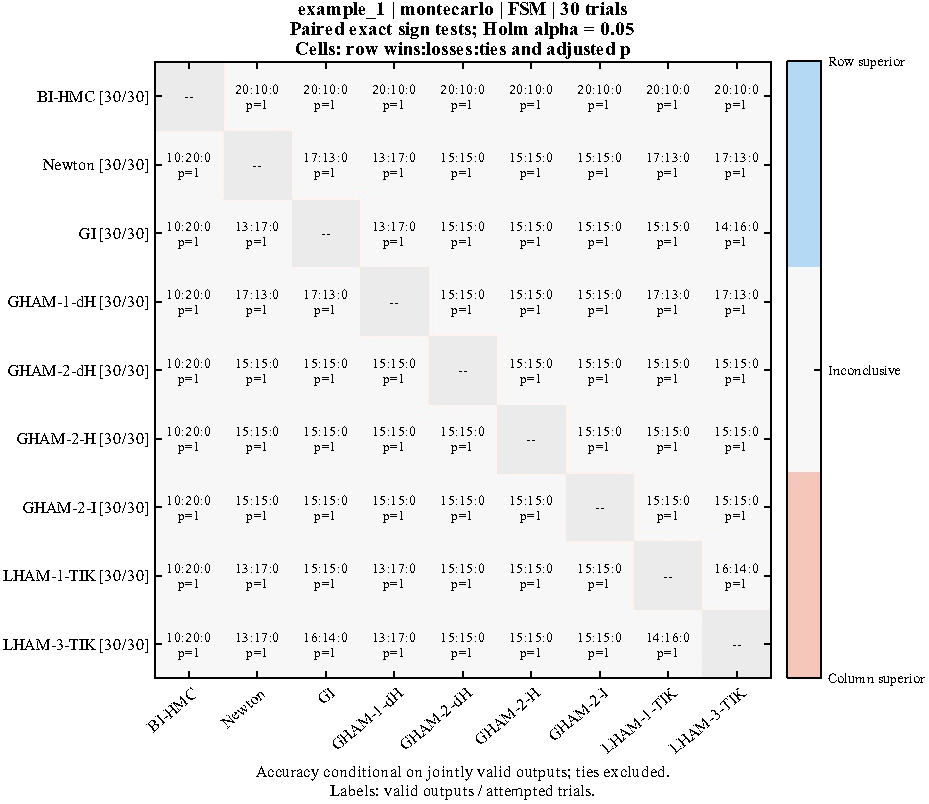
\includegraphics[width=\linewidth,height=.77\textheight,keepaspectratio]{output/experimental_statistics/parameter_error_wins_example_1_montecarlo_fsm.pdf}
\caption{Final-parameter-error comparison matrix for Example 1/FSM, 30 independent Monte Carlo records. Blue cells favor the row method and red cells favor the column method after Holm correction ($\alpha=0.05$); white cells are inconclusive. Paired cells show row wins:losses:ties and $p_{\rm H}$. Cells marked RS use independent rank-sum tests and show $\widehat A_{\rm row,col}$ and $p_{\rm H}$. Grey diagonal or NA entries are not tests.}
\label{fig:expstats_wins_example_1_montecarlo_fsm}
\end{figure}
\begin{figure}[p]
\centering
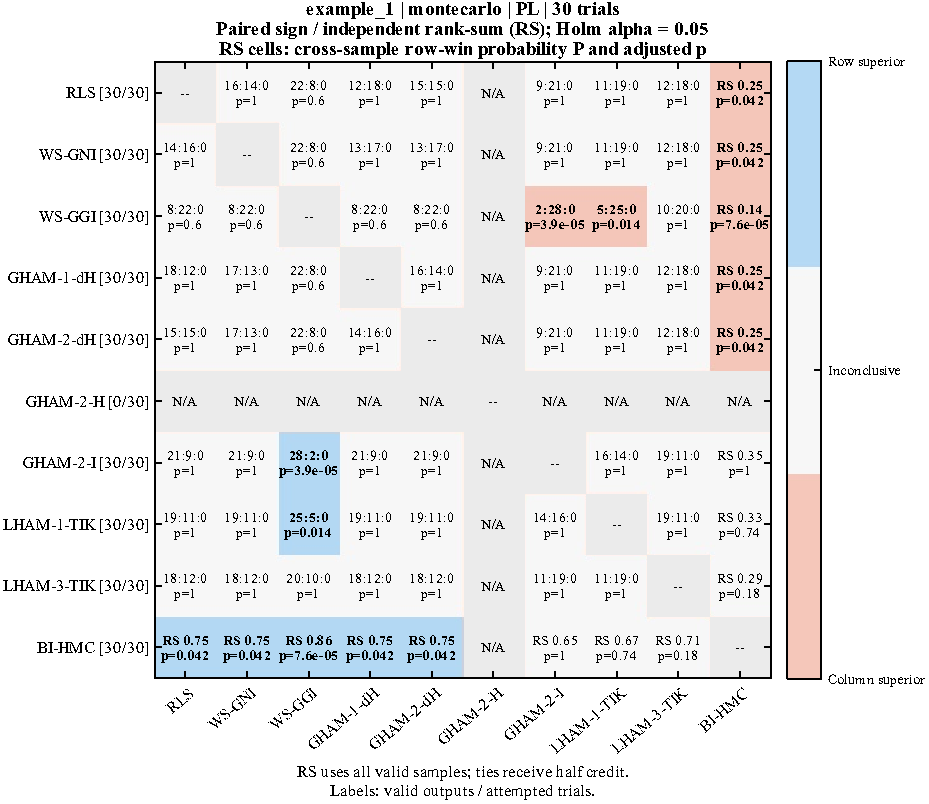
\includegraphics[width=\linewidth,height=.77\textheight,keepaspectratio]{output/experimental_statistics/parameter_error_wins_example_1_montecarlo_pl.pdf}
\caption{Final-parameter-error comparison matrix for Example 1/PL, 30 independent Monte Carlo records. Blue cells favor the row method and red cells favor the column method after Holm correction ($\alpha=0.05$); white cells are inconclusive. Paired cells show row wins:losses:ties and $p_{\rm H}$. Cells marked RS use independent rank-sum tests and show $\widehat A_{\rm row,col}$ and $p_{\rm H}$. Grey diagonal or NA entries are not tests.}
\label{fig:expstats_wins_example_1_montecarlo_pl}
\end{figure}
\begin{figure}[p]
\centering
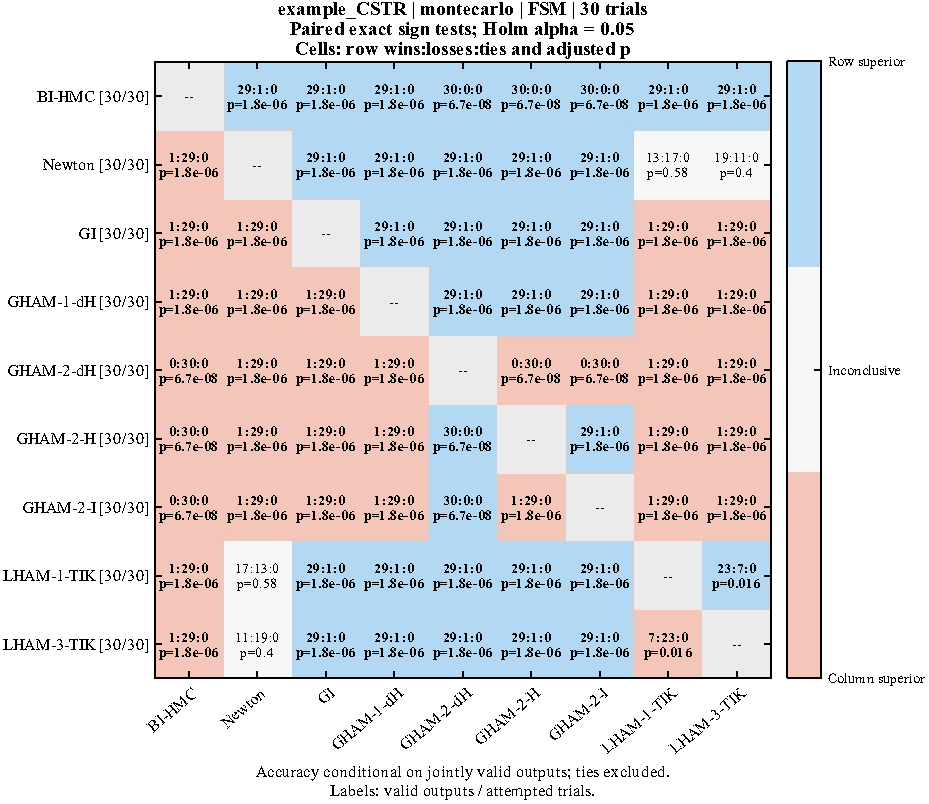
\includegraphics[width=\linewidth,height=.77\textheight,keepaspectratio]{output/experimental_statistics/parameter_error_wins_example_cstr_montecarlo_fsm.pdf}
\caption{Final-parameter-error comparison matrix for CSTR/FSM, 30 independent Monte Carlo records. Blue cells favor the row method and red cells favor the column method after Holm correction ($\alpha=0.05$); white cells are inconclusive. Paired cells show row wins:losses:ties and $p_{\rm H}$. Cells marked RS use independent rank-sum tests and show $\widehat A_{\rm row,col}$ and $p_{\rm H}$. Grey diagonal or NA entries are not tests.}
\label{fig:expstats_wins_example_cstr_montecarlo_fsm}
\end{figure}
\begin{figure}[p]
\centering
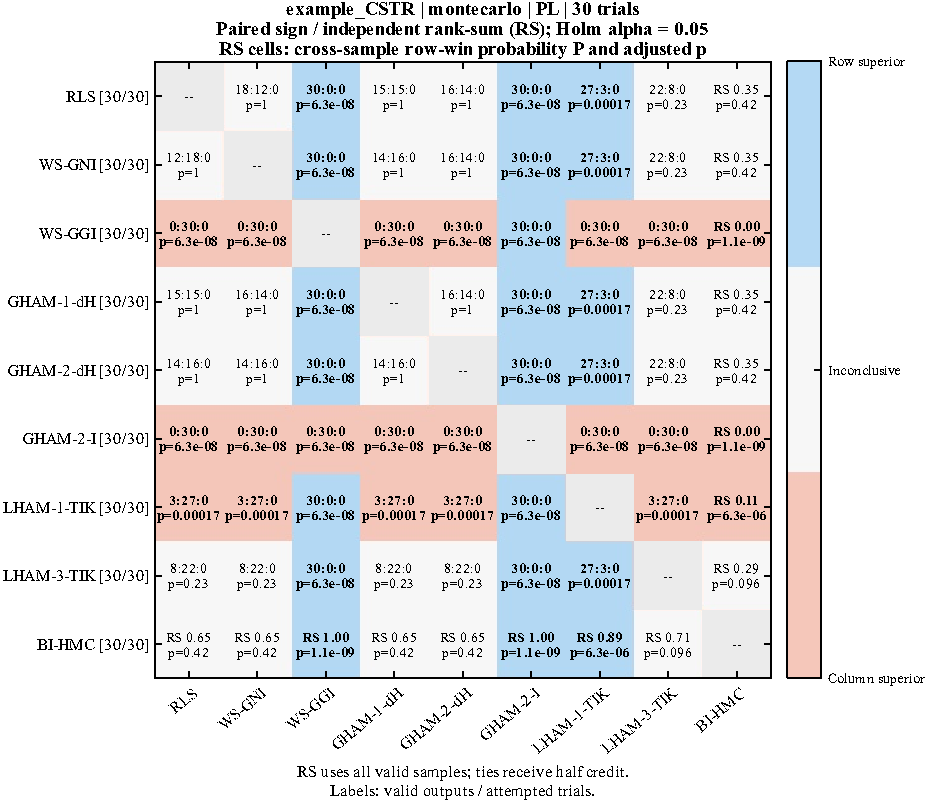
\includegraphics[width=\linewidth,height=.77\textheight,keepaspectratio]{output/experimental_statistics/parameter_error_wins_example_cstr_montecarlo_pl.pdf}
\caption{Final-parameter-error comparison matrix for CSTR/PL, 30 independent Monte Carlo records. Blue cells favor the row method and red cells favor the column method after Holm correction ($\alpha=0.05$); white cells are inconclusive. Paired cells show row wins:losses:ties and $p_{\rm H}$. Cells marked RS use independent rank-sum tests and show $\widehat A_{\rm row,col}$ and $p_{\rm H}$. Grey diagonal or NA entries are not tests.}
\label{fig:expstats_wins_example_cstr_montecarlo_pl}
\end{figure}
